\documentclass[tikz,border=12pt]{standalone}
\usepackage[T1]{fontenc}
\usepackage{tgheros}
\usepackage{sfmath}
\usepackage{amsmath}
\usepackage{amssymb}
\usepackage{fontawesome5}
\usepackage{tikz}
\usetikzlibrary{arrows.meta,positioning,shapes.geometric,fit,backgrounds,calc}
\usepackage{xcolor}

\renewcommand{\familydefault}{\sfdefault}

% Academic Semantic Palette
\definecolor{harvardcrimson}{HTML}{A51C30}
\definecolor{ethdarkblue}{HTML}{1F407A}
\definecolor{ethblue}{HTML}{215CAF}
\definecolor{ethpetrol}{HTML}{007A87}
\definecolor{ethbronze}{HTML}{B87333}
\definecolor{ethpurple}{HTML}{5B4B8A}
\definecolor{ethslate}{HTML}{475569}
\definecolor{cardbg}{HTML}{F8FAFC}
\definecolor{cardborder}{HTML}{CBD5E1}
\definecolor{safeTeal}{HTML}{10B981}
\definecolor{proposalAmber}{HTML}{C98218}

\begin{document}
\begin{tikzpicture}[
  font=\sffamily,
  >=Stealth,
  gatecard/.style={
    draw=cardborder,
    fill=cardbg,
    rounded corners=4pt,
    line width=0.8pt,
    text width=1.95in,
    minimum height=2.35in,
    inner sep=7pt,
    align=center,
    anchor=north
  }
]

  % Title Banner
  \node[draw=ethdarkblue, fill=ethdarkblue!5, rounded corners=5pt, line width=1pt, text width=8.80in, inner sep=7pt, align=center] (title) at (4.40in, 0) {
    {\normalsize\bfseries\color{ethdarkblue}\faIcon{filter}\;\; THE 3-GATE MORPHOLOGICAL REACHABILITY \& SINGULARITY VALIDATOR}\\[2pt]
    {\scriptsize\color{ethslate}Screening Untrusted Stochastic VLM Proposals Before Committing Downstream Motion Trajectories}
  };

  % Input: Untrusted VLM Proposal
  \node[draw=proposalAmber, fill=proposalAmber!10, rounded corners=4pt, line width=1pt, text width=1.50in, minimum height=2.35in, inner sep=7pt, align=center, anchor=north] (input) at (0, -0.65in) {
    {\scriptsize\bfseries\color{proposalAmber}\faIcon{brain}\; UNTRUSTED PROPOSAL}\\[4pt]
    {\small\bfseries VLM Semantic Intent}\\[6pt]
    \rule{0.9\linewidth}{0.3pt}\\[6pt]
    \raggedright
    {\tiny\textbf{\color{ethdarkblue}Pose:} $T_{\text{target}}^{\text{world}} \in SE(3)$}\\[4pt]
    {\tiny\textbf{\color{ethdarkblue}Coord:} $p_{\text{target}} \in \mathbb{R}^3$}\\[4pt]
    {\tiny\textbf{\color{ethdarkblue}Aperture:} $d_{\text{grasp}}$}\\[4pt]
    {\tiny\textbf{\color{ethdarkblue}Confidence:} $p_{\text{sem}} \ge 0.75$}\\[8pt]
    \centering
    \rule{0.9\linewidth}{0.3pt}\\[4pt]
    {\tiny\color{ethslate}Stochastic prediction from 2D pixels}
  };

  % Gate 1: Workspace Envelope
  \node[gatecard, draw=ethblue!80] (g1) at (2.05in, -0.65in) {
    {\scriptsize\bfseries\color{ethblue}\faIcon{expand-arrows-alt}\; GATE 1}\\[3pt]
    {\small\bfseries Workspace Envelope}\\[4pt]
    {\scriptsize\color{ethslate}Geometric Feasibility}\\[6pt]
    \rule{0.9\linewidth}{0.3pt}\\[6pt]
    \raggedright
    {\tiny\textbf{\color{ethdarkblue}Reach:} $\|p_{\text{target}} - p_{\text{base}}\| \le R_{\text{max}}$}\\[3pt]
    {\tiny\textbf{\color{ethdarkblue}Floor:} $z_{\text{target}} \ge z_{\text{table\_min}}$}\\[3pt]
    {\tiny\textbf{\color{ethdarkblue}Joint Bounds:} $q_{\text{min}} \le q \le q_{\text{max}}$}\\[3pt]
    {\tiny\textbf{\color{ethblue}IK Solver:} Analytical / Damped LS}\\[6pt]
    \centering
    \rule{0.9\linewidth}{0.3pt}\\[4pt]
    {\tiny\color{ethslate}Rejects points outside physical arm reach}
  };

  % Gate 2: Singularity & Manipulability
  \node[gatecard, draw=ethpetrol!80] (g2) at (4.30in, -0.65in) {
    {\scriptsize\bfseries\color{ethpetrol}\faIcon{tachometer-alt}\; GATE 2}\\[3pt]
    {\small\bfseries Singularity Filter}\\[4pt]
    {\scriptsize\color{ethslate}Jacobian Conditioning}\\[6pt]
    \rule{0.9\linewidth}{0.3pt}\\[6pt]
    \raggedright
    {\tiny\textbf{\color{ethdarkblue}Condition:} $\kappa(J) = \frac{\sigma_{\text{max}}}{\sigma_{\text{min}}} \le 50.0$}\\[3pt]
    {\tiny\textbf{\color{ethdarkblue}Manipulability:} $w = \sqrt{\det(J J^T)} \ge w_{\text{min}}$}\\[3pt]
    {\tiny\textbf{\color{ethdarkblue}Joint Velocity:} $\|\dot{q}\| = \|J^{-1} \dot{x}\| \le \dot{q}_{\text{max}}$}\\[3pt]
    {\tiny\textbf{\color{ethpetrol}Safety Margin:} Non-zero nullspace}\\[6pt]
    \centering
    \rule{0.9\linewidth}{0.3pt}\\[4pt]
    {\tiny\color{ethslate}Prevents infinite joint velocity spikes}
  };

  % Gate 3: Payload & Gravity Torque
  \node[gatecard, draw=ethpurple!80] (g3) at (6.55in, -0.65in) {
    {\scriptsize\bfseries\color{ethpurple}\faIcon{weight-hanging}\; GATE 3}\\[3pt]
    {\small\bfseries Static Torque Limits}\\[4pt]
    {\scriptsize\color{ethslate}Actuator Thermal Safety}\\[6pt]
    \rule{0.9\linewidth}{0.3pt}\\[6pt]
    \raggedright
    {\tiny\textbf{\color{ethdarkblue}Gravity Load:} $\tau_{\text{grav}}(q) \le \tau_{\text{cont}}$}\\[3pt]
    {\tiny\textbf{\color{ethdarkblue}Payload Wrench:} $J(q)^T F_{\text{load}} \le \tau_{\text{margin}}$}\\[3pt]
    {\tiny\textbf{\color{ethdarkblue}Thermal Rise:} $T_{\text{motor}} < 85^\circ\text{C}$}\\[3pt]
    {\tiny\textbf{\color{ethpurple}Current Draw:} $I_{\text{phase}} \le I_{\text{continuous}}$}\\[6pt]
    \centering
    \rule{0.9\linewidth}{0.3pt}\\[4pt]
    {\tiny\color{ethslate}Guards motor windings against stall burn}
  };

  % Connecting Arrows between Gates
  \draw[->, line width=1.1pt, draw=ethslate] (input.east) -- (g1.west);
  \draw[->, line width=1.1pt, draw=ethslate] (g1.east) -- (g2.west);
  \draw[->, line width=1.1pt, draw=ethslate] (g2.east) -- (g3.west);

  % Bottom Verdict Boxes
  \node[draw=safeTeal, fill=safeTeal!10, rounded corners=4pt, line width=1pt, text width=4.15in, inner sep=6pt, anchor=north] (pass) at (2.10in, -3.20in) {
    {\scriptsize\bfseries\color{safeTeal}\faIcon{check-circle}\;\; ALL GATES PASSED: ISSUE INTENT LEASE ($\mathcal{L}_{\text{intent}}$)}\\[2pt]
    {\tiny\color{ethdarkblue}Commit validated 3D target frame and workspace envelope to System 1.5 Trajectory Planner}
  };

  \node[draw=harvardcrimson, fill=harvardcrimson!10, rounded corners=4pt, line width=1pt, text width=4.15in, inner sep=6pt, anchor=north] (fail) at (6.70in, -3.20in) {
    {\scriptsize\bfseries\color{harvardcrimson}\faIcon{times-circle}\;\; GATE FAILED: EMIT STRUCTURED ABSTENTION}\\[2pt]
    {\tiny\color{harvardcrimson}Revoke intent proposal; command Category 2 Safe Position Hold; prompt operator for clarification}
  };

  % Connecting lines to bottom verdicts
  \draw[->, line width=1pt, draw=safeTeal] (g2.south) -- ++(0, -0.15in) -| (pass.north);
  \draw[->, line width=1pt, draw=harvardcrimson] (g3.south) -- ++(0, -0.15in) -| (fail.north);

\end{tikzpicture}
\end{document}
